\section{Structured Low-Rank Matrix Formats}
\label{sec:matrix_formats}

In order to represent a matrix $A$ in a structured low-rank format, the corresponding cluster tree $\mathcal{T}$ needs to be constructed first. This is done by defining the index tree $\mathcal{I}$ over the row indices of $A$ and the index tree $\mathcal{J}$ over the column indices. The size of the leaves is determined by the aforementioned balance of  efficiency and accuracy, but in principle it can be any arbitrary number such that the index range is split at least once. Calculating the tensor product of these two trees then results in the cluster tree $\mathcal{T}$. In this tree, each child node represents a sub-block of the matrix $A$, while the root contains the full matrix. Note that there can not be an overlap between the children of a node and all the nodes on the same level represent a full vie of the matrix $A$.

Using this representation, it becomes possible to exploit the low-rank properties of submatrices from A. By traversing the tree from top to bottom (i.e. from the root downwards), a rank $k$ approximation can be created for each block. If the specified accuracy criterion is met, the block is replaced by a low-rank representation and all its children are deleted. If the error is still to high, further traversal down the tree will be necessary, performing the same check for the child nodes. When this process arrives at a leaf node and the desired accuracy is still not obtainable, the block will be stored as a dense matrix instead. An example of a resulting hierarchical matrix from a corresponding cluster tree is provided in Figure~\hyperref[fig:hierarchical_cluster]{\ref{fig:hierarchical_cluster}}.

\begin{figure}[h]
    \centering
    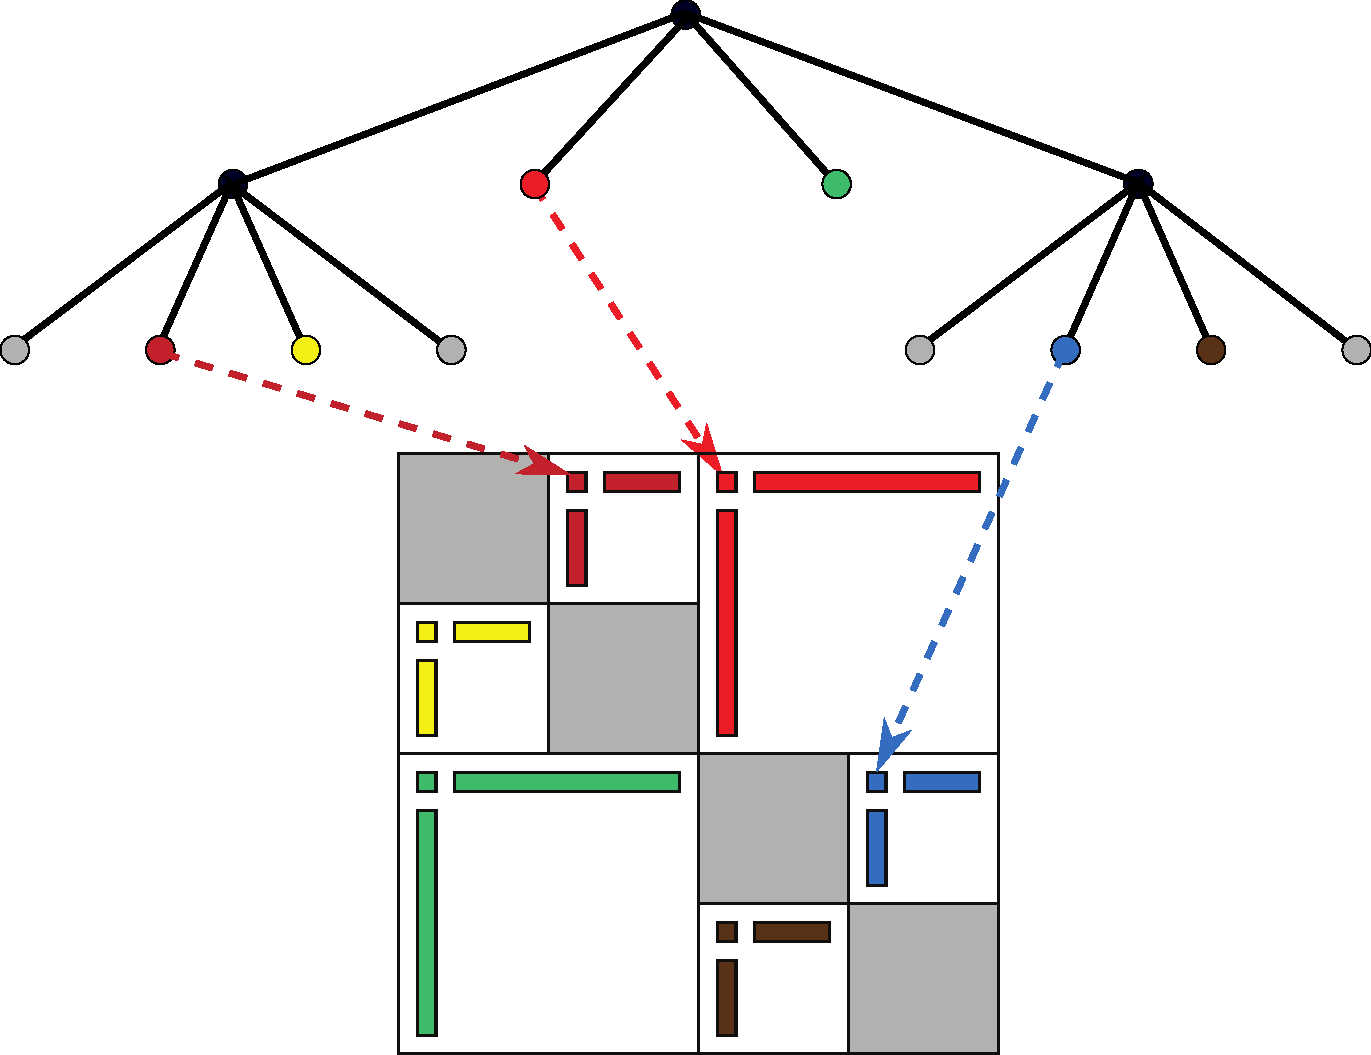
\includegraphics[width=0.9\linewidth]{chapters/4_hierarchical_matrices/figures/hierarchical_cluster.pdf}
    \caption[Hierarchical Matrix from Cluster Tree]{Example of a hierarchical matrix obtained from a corresponding cluster tree. The grey blocks denote dense blocks while the colored ones are low-rank approximations. Tree nodes and their corresponding matrix blocks share the same color (some example connections are illustrated with dotted lines).}
    \label{fig:hierarchical_cluster}
\end{figure}

Note that the process described is actually too expensive in practice, since low-rank approximations are calculated for all blocks, before deciding whether or not it is an appropriate representation for that block. Thus the result might be discarded in many cases, wasting a lot of computational effort. Hence it is more common to specify whether or not a block can be approximated beforehand, by means of an \textit{admissibility condition}. In the most general case, this admissibility condition is a Boolean function such that:
\begin{equation}
\label{eqn:admissibility}
    admissible: \mathcal{P}(I)\times \mathcal{P}(J) \rightarrow \{true, false\}
\end{equation}

\noindent $\mathcal{P}()$ denotes the power set, which is the set of all index subsets. In this sense, the admissibility condition decides whether or not a block of the matrix is approximated based on the corresponding index set (i.e. a decision is made for each node). According to \cite{hackbusch_hierarchical_2015}, such a mapping has to satisfy two general properties:
\begin{enumerate}
    \item Monotonicity: All children of an admissible block must be admissible as well.
    \item Symmetry: Provided that $I=J$, if $\{I\#x,J\#y\}$ is admissible, then $\{I\#y,J\#x\}$ is also admissible.
\end{enumerate}

\noindent According to \cite{hackbusch_hierarchical_2004}, there are two general types of admissibility. \textit{Weak} admissibility, where only blocks that cross the diagonal of the matrix are not admissible, and \textit{strong} admissibility (also referred to as standard admissibility, because it was the one originally proposed). Strong admissibility allows for dense blocks that are not on the diagonal, approximating blocks that are off the tri-diagonal.

Different kinds of structured low-rank approximations can be distinguished depending on this admissibility, the structure of the cluster tree and the storage representation. The characteristics of the specific formats, together with their advantages and disadvantages will discussed in the following sections.

\subsection{Block Low-Rank (BLR) Matrix}
\label{sec:blr}

The block low-rank storage format has been proposed by \cite{amestoy_improving_2015} as a specialized case of a hierarchical matrix that provides more flexibility and is easier to use/implement. It basically avoids recursion on sub-blocks by only splitting the matrix on the top level. In terms of the cluster tree $\mathcal{T}$, this is equivalent to having all the leaves on the same level (i.e. fixed depth of the tree), which additionally guarantees that all submatrices have the same size. Any admissibility condition can be applied to this type of matrix and an exemplary BLR matrix with weak admissibility is given in Figure~\hyperref[fig:blr]{\ref{fig:blr}}.

\begin{figure}[h]
    \centering
    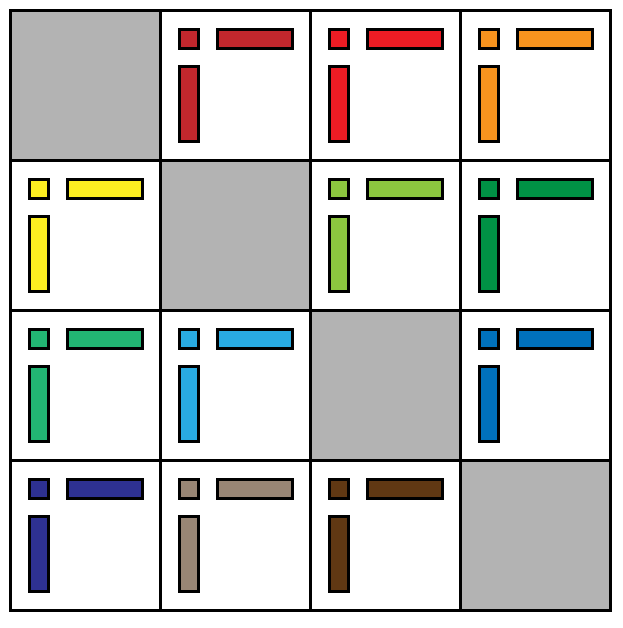
\includegraphics[width=0.6\linewidth]{chapters/4_hierarchical_matrices/figures/BLR.pdf}
    \caption[Block Low-Rank Matrix]{Example of a BLR matrix with weak admissibility. All blcoks are of equal size, with off-diagonal blocks being approximated by low-rank factorizations.}
    \label{fig:blr}
\end{figure}

The restrictions on the cluster tree imposed by this format have many favourable consequences. First, since all the blocks are on the same level, the matrix can be processed sequentially in a block-by-block fashion and does not need to rely on recursion at all. Being of equal size furthermore facilitates processing since all blocks can be handled in the same way. Second, interactions between block are well defined and efficient. Blocked variants of traditional matrix algorithms are available in many numerical libraries (e.g. \cite{anderson_lapack_1999} and are known to perform better than their element-wise counterparts on modern computer architectures. Hence matrix operations on BLR matrices can be performed relatively easy with similar procedures (all that is left is to define the interactions of the low-rank plots). Third, due to the aforementioned reasons, load balancing on parallel implementations is greatly simplified and the overhead of constructing the low-rank representation remains low (see \cite{amestoy_improving_2015}). 

On the other side, as a drawback of the simple tree structure, matrix operations conducted with this format are generally more expensive than those of the other formats that will be introduced later on. BLR matrix-matrix multiplication, for example, can be performed in $\mathcal{O}(n^2)$. While this is faster than the normal dense computations, it is still considerably slower than the (almost) linear complexity achieved by other representations. Arguably, the most interesting operation in the context of linear solvers is the LU factorization, and a detailed analysis by \cite{amestoy_complexity_2017}, shows an upper bound of $\mathcal{O}(n^2)$ as well. Because the BLR structure employs a flat representation (i.e. all leaves are on the same level) instead of a hierarchical one, the number of blocks remains a fraction of the matrix size and thus limits its scalability.

In order to bridge the gap to hierarchical approaches, while maintaining the ease of usage of the BLR format, an extension called \textit{multilevel BLR} (MBLR) was introduced by \cite{amestoy_bridging_2019}. The simple idea behind this proposal is to allow for multiple levels (i.e. a hierarchy) within the BLR structure, but at the same time fixing the number of levels to a certain parameter $\ell$. Hence it straightforward mechanism for managing the complexity, starting from $\ell=1$ (a normal BLR and thus $\mathcal{O}(n^2)$) up to an infinite number of levels $\ell=\infty$, which would achieve almost $\mathcal{O}(n)$. In contrast to the general partition rules mentioned in Section~\hyperref[sec:matrix_partition]{\ref{sec:matrix_partition}}, where the partition should contain as few blocks as possible, the number of children per node is asymptotically dependent on $n$ in the MBLR case. This is caused by the restriction on the number of levels $\ell$ the resulting structure for the case $\ell = 2$ is depicted in Figure~\hyperref[fig:mblr]{\ref{fig:mblr}}.

\begin{figure}[h]
    \centering
    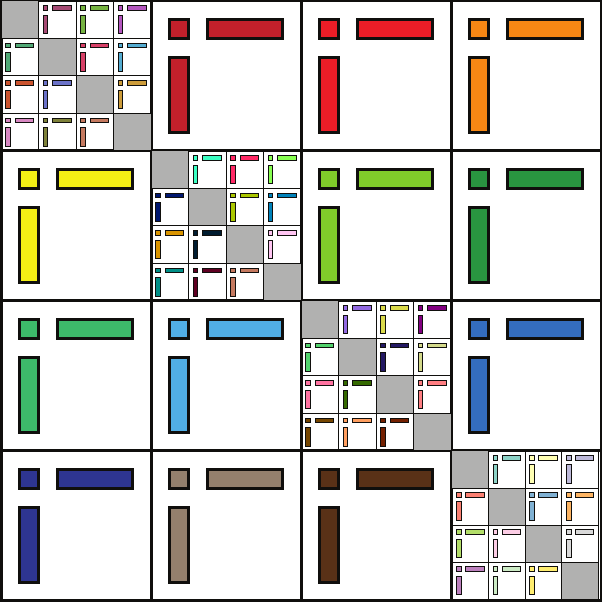
\includegraphics[width=0.6\linewidth]{chapters/4_hierarchical_matrices/figures/MBLR.pdf}
    \caption[Multilevel Block Low-Rank Matrix]{Example of a 2-level MBLR matrix with weak admissibility. In contrast to other hierarchical formats, the number of children per node governed by the block size $b$.}
    \label{fig:mblr}
\end{figure}

With regards to the expected accuracy of this representation, it has to be remarked that it depends entirely on the low-rank compression of the admissible blocks. This is the same for all hierarchical matrix formats, because the error induced by each compressed block is dependent on its rank $k$. Naturally, the quality of the approximation increases with the size of the rank, since the error of a full-rank representation is zero. Efficient computations, on the contrary, require a lower rank and thus there are two common ways to control this trade-off:
\begin{itemize}
    \item Fixing the rank $k$: This allows for fast and simple calculations, because the dimensions of the low-rank approximations are fixed. However, if the rank is chosen too low, some blocks might not be represented accurately.
    \item Fixing the error $\epsilon$: The rank can vary between blocks with each one selecting an appropriate $k$ in order to guarantee the maximal error $\epsilon$. The accuracy of the approximation can be controlled, but efficiency might suffer if the rank for some blocks is too large.
\end{itemize}

\subsection{BLR Matrix with Shared Bases (BLR\texorpdfstring{\textsuperscript{2}}{2})}
\label{sec:blr2}

The concept of shared (or in later cases nested) bases has been introduced together with hierarchical matrices (see \cite{hackbusch_hierarchical_2004}). It is based on the observation that for certain matrices arising from discretization of integral functions, the low-rank approximations sharing the same column or row range, are not entirely independent of each other. By finding appropriate cluster bases for such blocks, any admissible leaf block from $A \in \realx[I]{J}$ can be expressed as:
\begin{equation}
    A_{i,j}=U_i\cdot S_{i,j}\cdot V_j^T
\end{equation}

\noindent Hence, all blocks in the same row $i$ share the common basis $U_i$ and all blocks within the same column $j$ share the basis $V_j$. This reduces the storage requirement of an hierarchical representation drastically, since only the relatively small matrix $S_{i,j}$ needs to be maintained per block.

From an application point of view, a good example would be particle interactions in physics. Suppose those particles are sorted by some measure of spatial distance, then it is most likely that where will be several groups of particles that are closer to each other than to the rest. The interactions within such a group correspond to the dense parts in a hierarchical representation, while the interactions across groups are contained within the low-rank approximations. In this case, it is possible to summarize the outgoing interactions from group $i$ to all other groups via the row basis $U_i$. The incoming interactions can be summarized in a similar fashion giving rise to the row basis $V_i$. The full mathematical background to this idea can be found in \cite{hackbusch_h2-matrix_2002}.

For BLR matrices, this technique has been thoroughly explored by \cite{ashcraft_block_2020}, who used the 
name BLR\textsuperscript{2} to describe such a BLR format with shared bases. The process of who such a BLR\textsuperscript{2} matrix is constructed from an ordinary BLR representation will be outlined as an example on how such shared bases are obtained. Consider a BLR matrix $\Tilde{A}$, where each admissible block is approximated by a truncated SVD of the form:
\begin{equation}
    \Tilde{A}_{i,j} = U_{i,j}\cdot D_{i,j}\cdot V_{i,j}^T
\end{equation}

\noindent Suppose that the size of each block is given by $b$ such that $\Tilde{A}_{i,j} in \realx[b]{b}$ and a fixed rank $k$ is used for the representation, yielding $U_{i,j}, V_{i,j} \in \realx[b]{k}$ and $D_{i,j} \in \realx[k]{k}$. A shared basis for each column $c$ can be constructed via means of the QR factorization by combining the information from all admissible row blocks $i$:
\begin{equation}
  \left[
    \begin{array}{c|c|c}
      & & \\
      D_{1,c}\cdot V_{1,c} &\dots & D_{i,c}\cdot V_{i,c} \\
      & & \\
    \end{array}
  \right] = V_c
  \left[
    \begin{array}{c|c|c}
      & & \\
      E_{1,c}^T &\dots & E_{i,c}^T \\
      & & \\
    \end{array}
  \right]
\end{equation}

\noindent Analogously, the shared row basis (for any row $r$) can be obtained by combining the information from all admissible column blocks $j$:
\begin{equation}
  \left[
    \begin{array}{c|c|c}
      & & \\
      U_{r,1}\cdot D_{r,1} &\dots & U_{r,j}\cdot D_{r,j} \\
      & & \\
    \end{array}
  \right] = U_r
  \left[
    \begin{array}{c|c|c}
      & & \\
     F_{r,1} &\dots & F_{r,j} \\
      & & \\
    \end{array}
  \right]
\end{equation}

\noindent Note that for this process to be beneficial, the QR factorization must be combined with a compression scheme, such that the rank of the resulting basis accurately approximated. One efficient possibility would be a rank-revealing QR factorization as proposed by \cite{hong_rank-revealing_1992} or \cite{gu_efficient_1996}. Since a fixed rank $k$ was assumed in this example, the resulting bases are $U_{i}, V^T_{j} \in \realx[b]{k}$ and the matrix $S(i,j) \in \realx[k]{k}$ is given for each admissible block by:
\begin{equation}
    S_{i,j}=F_{i,j} \cdot E_{i,j}^T
\end{equation}

\begin{figure}[h]
    \centering
    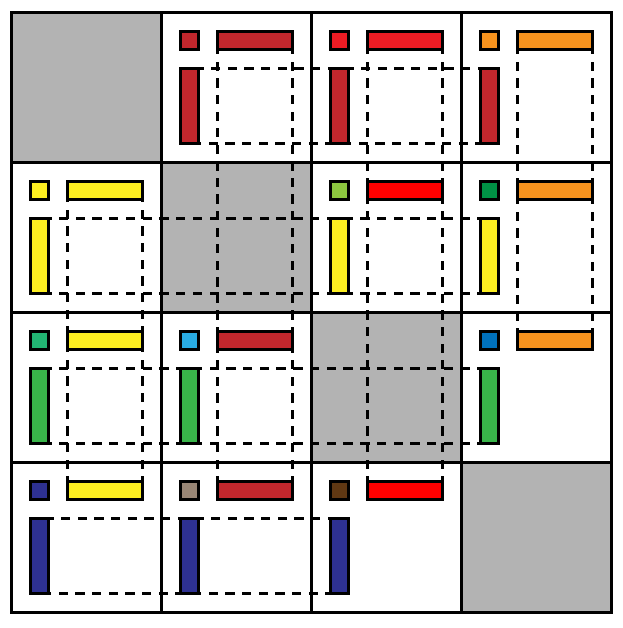
\includegraphics[width=0.6\linewidth]{chapters/4_hierarchical_matrices/figures/BLR_shared.pdf}
    \caption[BLR\texorpdfstring{\textsuperscript{2}}{2} Matrix]{Example of a BLR\textsuperscript{2} matrix with weak admissibility. The bases are now shared among the rows/columns of all admissible blocks (indicated by the same color).}
    \label{fig:blr_shared}
\end{figure}

On a practical note, the above assumption where the rank of the bases is equal to the rank of each low-rank approximation is hardly realistic in practice. The analysis by \cite{ashcraft_block_2020}, comparing the BLR and BLR\textsuperscript{2} format for different matrices suggest that in many cases, the storage requirements do not decrease when the approximation is based on an error threshold. Under weak admissibility, the rank of the shared bases becomes prohibitively large (with respect to the block size $b$), such that ordinary BLR matrices are actually more efficient. Employing strong admissibility criteria, however, changes the situation because less information needs to be represented in the bases. Under such circumstances a reduction in storage of about 30\% can be expected.


\subsection{Hierarchical Off-Diagonal Low-Rank (HODLR) Matrix}
\label{sec:hodlr}

In contrast to the BLR formats of the previous sections, HODLR is a true hierarchical format. Consequently, the leaves can be at different levels of the tree and calculations are a little bit more evolved, because they have to take this structure into account. Furthermore, the HOLDR format can be viewed as a general hierarchical matrix restricted to weak admissibility. As such, all non-diagonal blocks are approximated by low-rank representations. Is is usually represented by two binary index trees (to guarantee that sub-locks are as big as possible), with the depth of each tree depending on the matrix size $n$. The general structure of a HODLR matrix is presented in Figure~\hyperref[fig:hodlr]{\ref{fig:hodlr}}.

\begin{figure}[h]
    \centering
    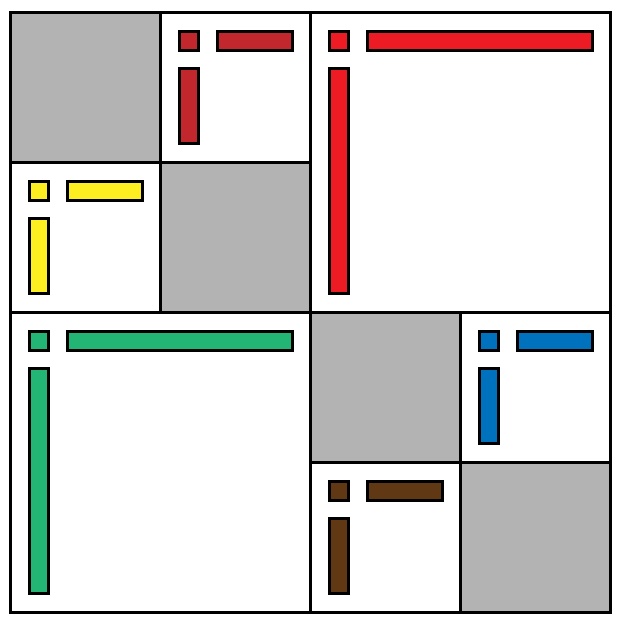
\includegraphics[width=0.6\linewidth]{chapters/4_hierarchical_matrices/figures/HODLR.pdf}
    \caption[Hierarchical Off-Diagonal Low-Rank Matrix]{Example of a HODLR matrix. Due to the weak admissibility condition, all off-diagonal blocks are low-rank approximations.}
    \label{fig:hodlr}
\end{figure}

With this kind of structure, it is no longer possible to process the matrix block sequentially, but instead it is necessary to traverse the tree in a \textit{depth-first} fashion, visiting the nodes in a certain order. Consider, for example the first level of the HODLR matrix in Figure~\hyperref[fig:hodlr]{\ref{fig:hodlr}}:
\begin{equation}
  A = 
  \left[
    \begin{array}{cc}
      A_1& A_2 \\
      A_3 & A_4 \\
    \end{array}
  \right]
\end{equation}

\noindent If a LU factorization of this matrix is desired, it would need to start at $A_1$ and invoke the operation recursively on all its sub-matrices, before any of the other blocks can be processed. After finishing $A_1$, $A_2$ and $A_3$ need to be updated before the Schur-complement for block $A_4$ can be calculated. However, all operations on $A_4$ would need to be done recursively again, due to its hierarchical structure. This dependencies between blocks of varying sizes make the underlying algorithms more complex than for the BLR case and load balancing more difficult on parallel architectures. Clearly, less work is associated with the blocks $A_2$ and $A_3$ and a simple distribution based on block sizes is not efficient for this type.

On the positive side, matrix-matrix computations and LU factorization can now be obtained in $\mathcal{O}(n\; log(n)$ operations and the same complexity is needed for constructing the HOLDR representation \cite{ambikasaran_fast_2016}. Even though this is the same as for general hierarchical matrices, the HODLR format generally benefits from more low-rank interactions. In other words, as long as the rank $k$ of the off-diagonal blocks remains small, this structure is the most beneficial in terms of storage and efficiency. However, guaranteeing, such a low-rank might lead to a larger error threshold for some matrices, resulting in a less accurate approximation.

An entire library dedicated to this format and providing the most common operations is available from \cite{ambikasaran_hodlrlib_2019}


\subsection{Hierarchical Semi-Separable (HSS) Matrix}
\label{sec:hss}

The hierarchical semi-seperable format is basically a shared bases extension of the HODLR structure. With respect to the hierarchical structure, however just sharing is not enough for this format, the bases must be \textit{nested} as well, since their sizes differ. Consider, for example the construction of a row basis for the the first level of the HODLR format. By looking at Figure~\hyperref[fig:hodlr]{\ref{fig:hodlr}}, it is evident that a common basis of the blocks $A_3$ and $A_4$ must provide a way to obtain the large green $U^{big}$ as well as the the two smaller blue and brown $U$s. Usually, this is solved by storing the basis in the smaller matrices, and then constructing the larger $U^{big}$ from those two via a so called \textit{transfer} matrix. Using this approach, only the relatively small transfer matrices need to be stored for the larger blocks, while the bases are entirely represented within the smallest level blocks. The resulting storage format is illustrated in Figure~\hyperref[fig:hss]{\ref{fig:hss}}.

\begin{figure}[h]
    \centering
    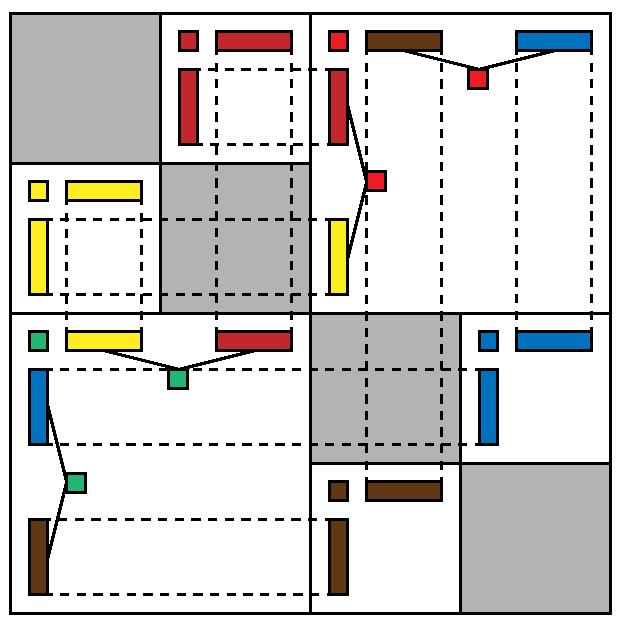
\includegraphics[width=0.6\linewidth]{chapters/4_hierarchical_matrices/figures/HSS.pdf}
    \caption[Hierarchical Semi-Separable Matrix]{Example of a HSS matrix. The low-rank approximations for the larger blocks are computed from the bases via transfer matrices (denoted as squares).}
    \label{fig:hss}
\end{figure}

The construction of such bases is slightly more evolved than for the BLR\textsuperscript{2} case, requiring the explicit calculation of $U^{big}$ and $V^{big}$ for each level. The necessary steps will be illustrated on the example of the HSS matrix with four diagonal blocks as shown in Figure~\hyperref[fig:hss]{\ref{fig:hss}}. This matrix has the following level one and two splittings:
\begin{equation}
  A = 
  \left[
    \begin{array}{cc}
      \iter[1]{D}_{11}& \iter[1]{A}_{12} \\
      \iter[1]{A}_{21} & \iter[1]{D}_{22} \\
    \end{array}
  \right]
  =     
  \left[
    \begin{array}{cccc}
      \iter[2]{D}_{11}& \iter[2]{A}_{12} & \iter[2]{A}_{13}& \iter[2]{A}_{14} \\
      \iter[2]{A}_{21} & \iter[2]{D}_{22} & \iter[2]{A}_{23}& \iter[2]{A}_{24} \\
      \iter[2]{A}_{31} & \iter[2]{A}_{32} & \iter[2]{D}_{33}& \iter[2]{A}_{34} \\
      \iter[2]{A}_{41} & \iter[2]{A}_{42} & \iter[2]{A}_{43}& \iter[2]{D}_{44} \\
    \end{array}
  \right]
\end{equation}

\noindent In this notation, the superscript marks the level and non-admissible blocks are denoted with $D$ (for diagonal) in order to avoid confusion. In order to calculate the $U$ and $V$ for the blocks in each  level, it is necessary to consider all admissible blocks in the same column/row \cite{xia_fast_2010}. Starting from the leaf level those are obtained for the first row and column by means of the QR factorization as follows:
\begin{equation}
  \left[
    \begin{array}{ccc}
      \iter[2]{A}_{12} & \iter[2]{A}_{13}& \iter[2]{A}_{14} \\
    \end{array}
  \right]
  = \iter[2]{U}_{12}
  \left[
    \begin{array}{ccc}
      \iter[2]{T}_{12} & \iter[2]{T}_{13}& \iter[2]{T}_{14} \\
    \end{array}
  \right]
\end{equation}

\noindent and
\begin{equation}
  \left[
    \begin{array}{c}
      \iter[2]{A}_{21} \\
      \iter[2]{A}_{31} \\
      \iter[2]{A}_{41} \\
    \end{array}
  \right]
  = V_{21}^{(2)T}
  \left[
    \begin{array}{ccc}
      \iter[2]{Z}_{21} \\
      \iter[2]{Z}_{31} \\
      \iter[2]{Z}_{41} \\
    \end{array}
  \right]
\end{equation}

\noindent Moving to the second row and column, the compression can be done without the previously calculated basis matrices, resulting in:
\begin{equation}
  \left[
    \begin{array}{ccc}
      \iter[2]{Z}_{21} & \iter[2]{A}_{23}& \iter[2]{A}_{24} \\
    \end{array}
  \right]
  = \iter[2]{U}_{21}
  \left[
    \begin{array}{ccc}
      \iter[B]{T}_{21} & \iter[2]{T}_{23}& \iter[2]{T}_{24} \\
    \end{array}
  \right]
\end{equation}

\noindent and
\begin{equation}
  \left[
    \begin{array}{c}
      \iter[2]{T}_{12} \\
      \iter[2]{A}_{32} \\
      \iter[2]{A}_{42} \\
    \end{array}
  \right]
  = V_{12}^{(2)T}
  \left[
    \begin{array}{ccc}
      \iter[2]{B}_{12} \\
      \iter[2]{Z}_{32} \\
      \iter[2]{Z}_{42} \\
    \end{array}
  \right]
\end{equation}

\noindent Thus, the matrix A becomes:
\begin{equation}
  \left[
    \begin{array}{cccc}
      \iter[2]{D}_{11}& \iter[2]{U}_{12}\iter[2]{B}_{12}V_{12}^{(2)T} & \iter[2]{U}_{12}\iter[2]{T}_{13}& \iter[2]{U}_{12}\iter[2]{T}_{14} \\
      \iter[2]{U}_{21}\iter[2]{B}_{21} V_{22}^{(2)T}& \iter[2]{D}_{22} & \iter[2]{U}_{21}\iter[2]{T}_{23}& \iter[2]{U}_{21}\iter[2]{T}_{24} \\
      \iter[2]{Z}_{31}V_{22}^{(2)T} & \iter[2]{Z}_{32}V_{12}^{(2)T} & \iter[2]{D}_{33}& \iter[2]{A}_{34} \\
      \iter[2]{Z}_{41}V_{22}^{(2)T} & \iter[2]{Z}_{42}V_{12}^{(2)T} & \iter[2]{A}_{43}& \iter[2]{D}_{44} \\
    \end{array}
  \right]
\end{equation}

\noindent Now the first level transfer matrices $\iter[1]{R}_{21}$ and $\iter[1]{W}_{12}$ can be obtained from merging and re-compressing the appropriate second level bases:
\begin{equation}
  \left[
    \begin{array}{cc}
      \iter[2]{T}_{13}& \iter[2]{T}_{14}  \\
      \iter[2]{T}_{23}& \iter[2]{T}_{24}  \\
    \end{array}
  \right]
  =  \iter[1]{R}_{21} \iter[1]{T}_{21}\text{,}\;\; \text{ and }\;\; 
  \left[
    \begin{array}{cc}
      Z_{31}^{(2)T}& Z_{41}^{(2)T}  \\
      Z_{32}^{(2)T}& Z_{42}^{(2)T}  \\
    \end{array}
  \right] = \iter[1]{W}_{12}Z_{12}^{(1)T} 
\end{equation}

\noindent Bases and transfer matrices for the other blocks can be obtained in an analogous fashion and in case of a deeper tree, the same process has to be repeated recursively on each level. A graphical interpretation of the above process is given in Figure~\hyperref[fig:nested_bases]{\ref{fig:nested_bases}}. The calculations follow the general algorithm outlined in \cite{xia_fast_2010}, but different approaches are possible (see, for example \cite{martinsson_fast_2011}. The construction of an HSS matrix is generally more costly than HODLR, with an complexity of $\mathcal{O}(n^2)$. However, as its main advantage, storage requirements can be reduced dramatically and for certain types of matrices almost linear scaling is achieved. Furthermore, there are algorithms which can solve linear system involving an HSS matrix in $\mathcal{O}(n)$ \cite{chandrasekaran_fast_2006}.

\begin{figure}[h]
    \centering
    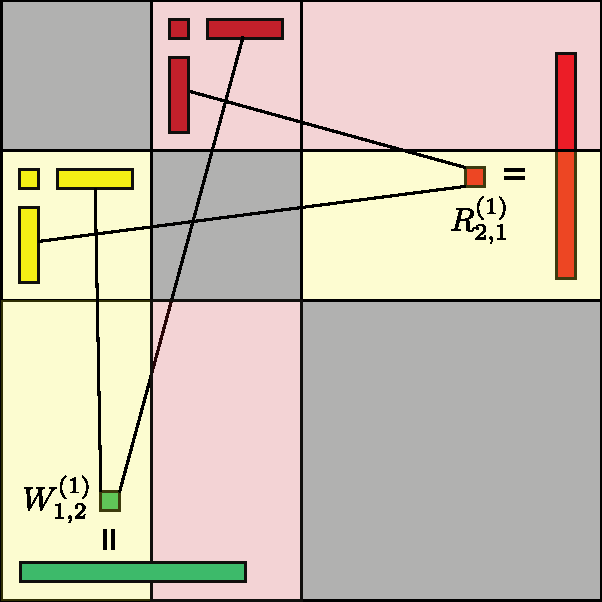
\includegraphics[width=0.6\linewidth]{chapters/4_hierarchical_matrices/figures/nested_basis.pdf}
    \caption[Nested Bases Construction]{Construction of the nested bases for the HSS format. $\iter[1]{R}_{21}$ and $\iter[1]{W}_{12}$ are the transfer matrices used to obtain $\iter[1]{U}_{21}$ $\iter[1]{V}_{21}$ from the bases stored at the leaf level.}
    \label{fig:nested_bases}
\end{figure}

\subsection{\texorpdfstring{$\mathcal{H}$}{H}-matrix}
\label{sec:h_matrix}
The generalization of the HODLR format to arbitrary admissibility conditions is called a $\mathcal{H}$(ierarchical)-matrix. This type is often used in combination with strong admissibility, but in principle, any function formulated according to Equation~\hyperref[eqn:admissibility]{\ref{eqn:admissibility}} can be employed. However, while less admissible blocks generally lead to a greater accuracy of the representation, more storage and computing power is necessary to process these dense blocks. Therefore, if the underlying problem admits it (for example in \cite{ambikasaran_fast_2016}), HODLR matrices are often preferred since they keep the number of dense blocks at a minimum. If the rank of the off-diagonal blocks remains low, weak admissibility is more efficient and high performance can be expected.

At the same time, both BLR and BMLR are also special cases of a hierarchical matrix, but with a restriction applied to the cluster tree (by limiting the number of levels). In principle, this storage format admits for any shape of the cluster tree, creating deeper or shallower matrices depending on the number of children. In combination with the admissibility condition, this leads to a wide variety of possible $\mathcal{H}$-matrix shapes. Of course, not all of them are desirable because they can severely limit the performance and bad choices of depth, split and admissibility might induce a huge overhead. Binary trees are often preferred since they guarantee a low number of blocks, and Figure~\hyperref[fig:h_matrix]{\ref{fig:h_matrix}} illustrates the resulting matrix with strong admissibility condition.

\begin{figure}[h]
    \centering
    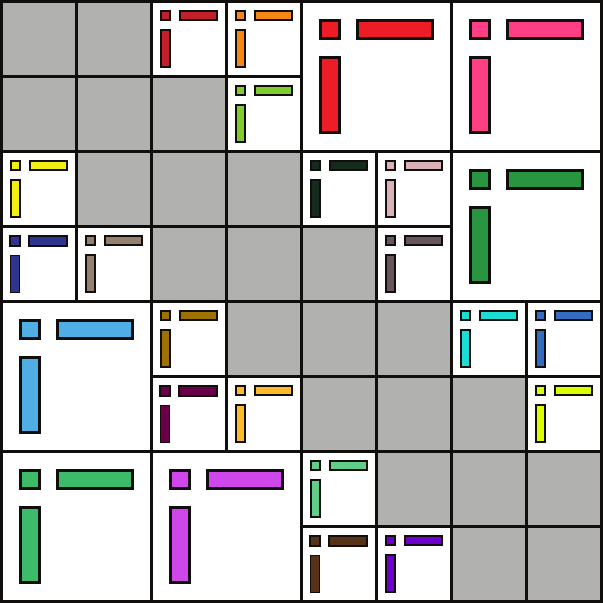
\includegraphics[width=0.6\linewidth]{chapters/4_hierarchical_matrices/figures/H_matrix.pdf}
    \caption[\texorpdfstring{$\mathcal{H}$}{H}-matrix]{$\mathcal{H}$-matrix with strong admissibility. Only blocks off the tri-diagonal are approximated by low-rank representations.}
    \label{fig:h_matrix}
\end{figure}

Due to the flexibility of the format, it is applicable to a wide range of problems, while at the same time requiring a deep understanding of its underlying structure. Suitable low-rank blocks must be located and approximated based on an admissibility condition built from prior knowledge of the matrix structure, which, also determines the leaf-size of the cluster tree. This information must be available before building the actual matrix, since the workload associated with a dynamic detection of the structure is too expensive for real world problems. Thus, the parameters need to be selected carefully, because the incorporated assumptions will have a large impact on the result, in case they are not met by the actual matrix. A fixed-rank implementation, for example will likely induce large errors if the admissible blocks are not truly low-rank (causing the low-rank approximation to be very inaccurate). Similarly, if an error-threshold is used instead, the rank for such a block will be close to $n$, making the processing very inefficient (but accuracy will be maintained).   

Therefore, while being a powerful tool in theory, having domain expertise is essential when dealing with hierarchical matrices as they do not provide a simple one-size-fits-all solution. In principle, the creation of the $\mathcal{H}$-matrix creates and additional overhead that must be amortized by the efficiency of the format. Careful construction play a vital role in this concept, and any knowledge available should be used to optimize this part of the process.


\subsection{\texorpdfstring{$\mathcal{H}^2$}{H2}-matrix}
\label{sec:h2_matrix}

The $\mathcal{H}^2$ storage format complements the field of hierarchical matrices by extending it to the concept of nested/shared bases. Much like HODLR and BLR are special types of $\mathcal{H}$-matrices, the  $\mathcal{H}^2$ layout can be considered as the parent class to instances like HSS and BLR\textsuperscript{2}. It is defined for arbitrary cluster trees and admissibility conditions, built around the core concept of sharing common bases for low-rank sub-matrices. Hence, computations can be done even more efficiently and storage requirements are reduced as well. They are known to work very well for the integral operators of classical potential theory and are also applicable to solution operators of elliptic partial differential equations \cite{borm_h2-matrix_2006}.

The construction mechanism is almost identical to the process described for HSS-matrices in Section~\hyperref[sec:hss]{\ref{sec:hss}}, with the only difference being that weak admissibility is not mandatory. As a consequence, there might be more than one dense block per row/column, possibly resulting in a lower rank of the shared bases. This is because all dense blocks are disregarded when building the shared bases resulting in less column/rows that need to be compressed. This becomes immediately evident when comparing the HSS (see Figure~\hyperref[fig:hss]{\ref{fig:hss}}) to the $\mathcal{H}^2$ with strong admissibility depicted in Figure~\hyperref[fig:h2_matrix]{\ref{fig:h2_matrix}}. For the same matrix size $n$, the block structure becomes more fine-grained and one additional leaf-size block is excluded from the basis in most cases.

\begin{figure}[h]
    \centering
    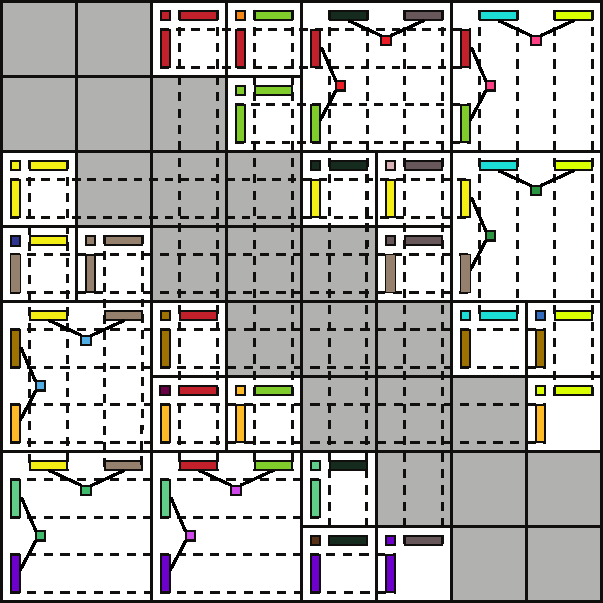
\includegraphics[width=0.6\linewidth]{chapters/4_hierarchical_matrices/figures/H2_matrix.pdf}
    \caption[\texorpdfstring{$\mathcal{H}^2$}{H2}-matrix]{$\mathcal{H}^2$-matrix with strong admissibility. Only blocks off the tri-diagonal are approximated by low-rank representations.}
    \label{fig:h2_matrix}
\end{figure}

As a consequence, if the upper and lower blocks of the tri-diagonal have a large rank, that information does not need to be compressed into the shared bases, probably resulting in a leaner structure and a lower rank of the bases themselves. In such a case, the $\mathcal{H}^2$ format can be much more efficient than HSS because it prevents the bases from growing large. Examples and a detailed discussion about this phenomenon (comparing BLR and BLR\textsuperscript{2}, but the same arguments apply to all shared-bases formats) can be found in \cite{ashcraft_block_2020}. Note that this does not necessarily mean that those blocks are not low-rank, just that there rank is considerably larger than that of the other block in the same row or column. Therefore, even if the underlying structure admits weak admissibility, a $\mathcal{H}^2$-matrix might be more efficient than HSS in some cases.

However, the most remarkable property of $\mathcal{H}^2$ matrices, is that they reduce the storage complexity to $\mathcal{O}(n)$. Furthermore, algorithms are available are able to perform matrix-matrix multiplication and LU factorization in linear complexity (see \cite{borm_h2-matrix_2006}). Even though the involved arithmetic operations are generally more evolved than for regular $\mathcal{H}$- matrices, the nested/shared bases variants have the advantage in terms of speed, making them the most efficient storage format based on approximate low-rank representations.